\documentclass[12pt,a4paper]{extreport}
\usepackage{epsfig}
\usepackage{moreverb}
\usepackage{color}
\usepackage{fancyhdr,a4wide}
\usepackage{makeidx}
\usepackage{amssymb,amsmath}
\usepackage{multirow}
\usepackage{fancyvrb}
\usepackage{listings} 
\usepackage[ngerman,english]{babel}
\usepackage{graphicx}
\usepackage{float}
\usepackage[small,bf]{caption}
\usepackage{url}
% Define a new 'leo' style for the package that will use a smaller font.
\makeatletter
\def\url@leostyle{%
  \@ifundefined{selectfont}{\def\UrlFont{\sf}}{\def\UrlFont{\scriptsize\ttfamily}}}
\makeatother
% Now actually use the newly defined style.
\urlstyle{leo}
\usepackage[bookmarksnumbered,%
            pdffitwindow=true, %
            pdfstartview=Fit,%
            colorlinks=false,%
            pdfborder={0 0 0}]%
				{hyperref}
\usepackage{breakurl}
\usepackage{amssymb,amsmath}
\usepackage[nonumberlist,acronym,toc]{glossaries}
\usepackage{paralist}
\usepackage{calc}
\usepackage{lscape}
\usepackage{stmaryrd}
\usepackage[chapter]{algorithm}
\usepackage{algorithmic}
\usepackage{listings}
\usepackage{courier}
\lstset{
         basicstyle=\footnotesize\ttfamily, % Standardschrift
         numbers=left,               % Ort der Zeilennummern
         numberstyle=\tiny,          % Stil der Zeilennummern
         %stepnumber=2,               % Abstand zwischen den Zeilennummern
         numbersep=5pt,              % Abstand der Nummern zum Text
         tabsize=2,                  % Groesse von Tabs
         extendedchars=true,         %
         breaklines=true,            % Zeilen werden Umgebrochen
         keywordstyle=\color{red},
    		frame=b,         
         stringstyle=\color{white}\ttfamily, % Farbe der String
         showspaces=false,           % Leerzeichen anzeigen ?
         showtabs=false,             % Tabs anzeigen ?
         xleftmargin=17pt,
         framexleftmargin=17pt,
         framexrightmargin=5pt,
         framexbottommargin=4pt,
         showstringspaces=false      % Leerzeichen in Strings anzeigen ?        
}
\lstloadlanguages{% Check Dokumentation for further languages ...
         %[Visual]Basic
         %Pascal
         %C
         %C++
         %XML
         %HTML
         Java
 }
\usepackage{caption}
\DeclareCaptionFont{white}{\color{white}}
\DeclareCaptionFormat{listing}{\colorbox[cmyk]{0.43, 0.35, 0.35,0.01}{\parbox{\textwidth}{\hspace{15pt}#1#2#3}}}
\captionsetup[lstlisting]{format=listing,labelfont=white,textfont=white, singlelinecheck=false, margin=0pt, font={bf,footnotesize}}
\usepackage[all]{hypcap}

\makeglossaries
\newacronym{IR}{IR}{Information Retrieval}
\newacronym{LSA}{LSA}{Latent Semantic Analysis}
\newacronym{CMS}{CMS}{Content Management System}
\newacronym{LSI}{LSI}{Latent Semantic Indexing}
\newacronym{SVD}{SVD}{Singular Value Decomposition}
\newacronym{VSM}{VSM}{Vector Space Model}
\newacronym{WCC}{WCC}{Weighted Centroid Covering}
\newacronym{STC}{STC}{Suffix Tree Clustering}
\newacronym{HAC}{HAC}{Hierarchical Agglomerative Clustering}
\newacronym{OWL}{OWL}{Web Ontology Language}

% don't indent new paragraphs
\parindent 0pt

\hoffset+0.3in
\textwidth13cm
\textheight22cm

%\usepackage{graphicx}
\makeatletter
\def\ScaleIfNeeded{%
\ifdim\Gin@nat@width>\linewidth
\linewidth
\else
\Gin@nat@width
\fi
}
\makeatother

\pagestyle{headings}
\begin{document}
\clubpenalty = 10000
\widowpenalty = 10000 
\displaywidowpenalty = 10000

\newenvironment{summary}{\begin{quotation}\it\textbf{Summary.\space}}{\end{quotation}\vspace{0.3cm}}
\begin{titlepage}

% add the title page to pdf bookmarks
\pdfbookmark[0]{Titlepage}{title}

\begin{minipage}{1\linewidth}
\begin{flushright}
\begin{minipage}[h]{0.4\linewidth}

\includegraphics[height=2cm]{img/sts}
\end{minipage}
\hspace{0.5cm}
\begin{minipage}[h]{0.4\linewidth}

\includegraphics[height=2cm]{img/CoremediaLogo}
\end{minipage}\\
\bigskip
\Huge
\hrulefill\\
\bigskip
\begin{center}
Tag Cloud Control \\
by Latent Semantic Analysis\\
\end{center}
\hrulefill\\ 
\bigskip 
\bigskip
\large \textsc{Master's Thesis}\\
\medskip
\normalsize submitted by\\
\large
Angelina \textsc{Velinska}\\
\normalsize IMT\\
\end{flushright}
\end{minipage}

\vspace{2.5cm}

\begin{minipage}[b]{1\linewidth}
\begin{flushleft}

supervised by\\
\medskip
\large
Prof. Dr. rer. nat. habil.~Ralf \textsc{M\"oller}\\
Dipl. Ing. Sylvia \textsc{Melzer}\\
%\skip
\normalsize 
Software Systems Institute\\
\medskip

\large Prof. Dr.~Karl-Heinz \textsc{Zimmermann}\\
\normalsize Institute of Computer Technology\\
Hamburg University of Technology\\

\bigskip
\bigskip
\large
Dr.~Michael \textsc{Fritsch}\\
\normalsize 
CoreMedia AG\\
Hamburg\\



\end{flushleft}

\begin{center}
% Bottom of the page
\bigskip
\large
\textsc{Hamburg University of Technology}\\
{\large December, 2010} 
\end{center} 

\end{minipage}

\end{titlepage}

% include after creating the abstract
%\begin{abstract}

A short description of my work. 

\end{abstract}


% don't put page numbers on declaration and acknowledgement pages:
{\renewcommand{\thepage}{}
\pdfbookmark[0]{Declaration}{declaration}
\bigskip
\bigskip

\pagebreak\par
{\LARGE\noindent \textbf{Declaration}}\\

\bigskip
\bigskip

\noindent I declare that:\\

\medskip

This work has been prepared by myself, all literal or content based quotations are clearly pointed out, and no other sources or aids than the declared ones have been used.\\
\vspace{2cm}\\

\begin{flushright}
Angelina Velinska 
\end{flushright}

Hamburg \\
December, 2010 

\pagebreak 

%\pdfbookmark[0]{Acknowledgements}{acknowledgements}
\pagebreak\\
\vspace{14cm}\\

Thank you...



\pagebreak

}


% make figure names bold:
\makeatletter
\renewcommand{\fnum@figure}{\textbf{Figure~\thefigure}}
\makeatother

\pdfbookmark[0]{Contents}{contents}
\tableofcontents
\pdfbookmark[0]{List of figures}{figures}
\listoffigures
\listoftables
\listofalgorithms
\lstlistoflistings

\chapter{Introduction}
\label{sec:introduction}

Identifying the main concepts in texts is the subject of many research studies in the field of information retrieval and data mining. \\

This work investigates the implementation of Latent Semantic Analysis (LSA) for discovering the main concepts in texts, in order to present an overview of the text content in the form of a tag cloud.\\
\\
1. introductory words, why is this work being written \\
2. mention information retrieval, lsa, tag clouds - generally\\
3. mention cms ? document collections ? content ? \\
4. mention the work of david mugo \\
\\
During the last decade there have been constant optimizations in information retrieval effectiveness, making web search the preferred source of finding information. A substantial part of information retrieval deals with providing access to unstructured information in various domains. \gls{IR} refers to finding material (usually documents) of an unstructured nature (usually text) that satisfies an information need from within large collections (usually stored on computers) \cite{Mann08}. Many people today use methods from the field of IR when they use a search engine online, or search through their emails. In this context "unstructured data" refers to data which does not have a clear structure.\\

\gls{IR} technologies find wide application - in search engines, for browsing or filtering document collections, for further processing a set of retrieved documents. Before retrieval the documents are indexed, otherwise at each search, they would have to be scanned through for each query. The index maps the words or terms back to the documents where they occur. A method for document indexing, which is applied in this work, is called \gls{LSA}. It indexes the document collection by representing it as a reduced matrix of words and documents. \gls{LSA} representation improves \gls{IR} performance with respect to a basic problem of word-matching search - synonymy, or the case when more than one term describe the same concept. \\

While \gls{IR} deals with retrieval of documents, other systems manage content, such as documents. Content management includes a set of technologies and processes that support the creation, management and publication of content in any form or medium. Content may be documents, multi-media files, or any other file types that follow content lifecycle and require management. \gls{CMS} vary depending on their purpose and target environments - there are \gls{CMS} for the web, for enterprise, for mobile devices, as well as \gls{CMS} for managing collection of documents. \\

\section{Motivation and objective}
\label{sec:introduction:motandobj}  
A drawback of the classical \gls{LSA} implementation as an \gls{IR} method is the low precision of the returned results. A previous work by David Mugo \cite{mugo10} has investigated the improvement of \gls{LSA} precision performance by annotating the document collection and including the anotations used in \gls{LSA}. In his work, Mugo constructs a concept-document matrix from the annotations used, and concatenates it with the word-document matrix normally generated in \gls{LSA} process. The proposed solution, however, results in a slow speed of \gls{LSA}, and has left Mugo's hypothesis open. \\

Taking into consideration the results from Mugo's work, the current project has several objectives to reach. It will investigate the implementation of \gls{LSA} method for improving information retrieval in a domain-specific document management system with respect to context-based search. A further investigation will be made on improving the precision performance of \gls{LSA} method by using semantic annotations, and on finding an adequate way to present the results of \gls{LSA} as a tag cloud. And finally, it will be investigated how to use the tag cloud as a form of a relevance feedback to control \gls{LSA} method. \\

In the context of the stated objectives, semantic annotations are meta data annotations used to add information to unstructured data, or to the document collection. Semantic annotations are based on an ontology in our case, specifically developed for the domain of interest CoreMedia \gls{CMS}. Ontologies are used to capture some knowledge about a certain domain, by describing the concepts of the domain and the relationships between them. To further clarify the objectives, relevance feedback is an \gls{IR} technique, used to influence the retrieved results based on the user's preference. It allows the user to modify the initial tag cloud by selecting the most relevant words. The tag cloud is then re-generated from \gls{LSA} results with the relevance feedback posted as a query. \\

\section{Outline}
\label{sec:introduction:outline}
The reminder of this work is organized as follows. Chapter \ref{sec:docmanagsystem} describes in more detail what a document management system is, and provides an overview of the general structure of DocMachine 2.0, the \gls{CMS} deployed at CoreMedia AG. Chapter \ref{sec:semannot} presents the basic concepts of ontologies and document annotations based on ontologies. In Chapter \ref{sec:lsa} an overview of latent semantic analysis method is given, as well as an approach for improving \gls{LSA}'s precision by including semantic annotations in the method. Chapter \ref{sec:implementation} presents the prototype implementation and makes an evaluation of the results achieved in this work. And finally, conclusions are drawn in Chapter \ref{sec:conclusion}, along with some limitations of the current study and outlook for a future research.   \\ 

\chapter{Latent Semantic Analysis}
\label{sec:lsa}

%\begin{summary}
%The chapter gives a theoretical overview of \gls{LSA} in the context of its use in this work.
%\end{summary}
 
\section{Information Retrieval process}
\gls{IR} systems aim to satisfy user's information needs, by providing access to large collections of documents.  In a search application, the \gls{IR} process retrieves a set of documents which matches a given query. There are three basic processes which an \gls{IR} system has to support: to represent the content of the documents, to represent the user's information need, and to compare the two representations, based on a chosen similarity measure~(fig.~\ref{lsa:fig:ir_process}).
%
% IR process
%
\begin{figure}[htbp]
	\centering
	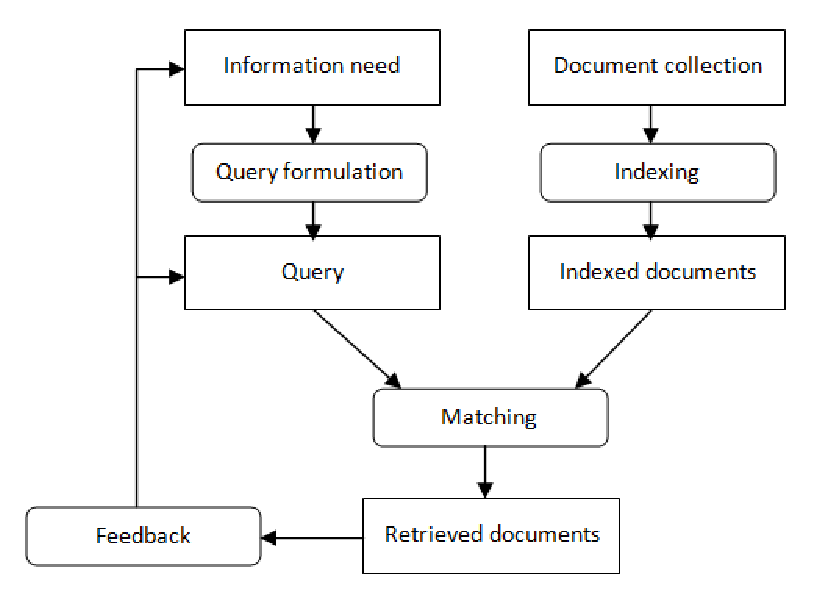
\includegraphics[scale=0.7]{img/IR} 
	\caption[Information Retrieval process]%
           {Information retrieval process, adapted from \cite{IRmodels09}. The information need of the user is formulated as a query, which is transformed in the chosen model of the \gls{IR} system. Documents from the collection are also represented according to the chosen model. Based on the implemented similarity measure, matching documents are identified. Finally, the retrieved results are presented to the user. If the user is not satisfied with the search results, the search query can be reformulated during feedback.}
\label{lsa:fig:ir_process}
\end{figure} 
Therefore, the first stage of constructing an \gls{IR} system is to extract information about the documents content, and implement a similarity measure, based on which documents and queries can be compared. Representing the documents is usually called the \textit{indexing process}. The comparison of the query against the document representations based on a chosen measure is called the \textit{matching process}.\\

\section{Document representation}
\label{sec:lsa:doc_repres}
In order to find documents which are similar to a given query, both documents and query have to be comparable, or have the same representation in the \gls{IR} system. Various models have been proposed for internal representation of documents and queries. The \textit{Boolean}, \textit{Vector space} and \textit{Probabilistic models} are popular \gls{IR} models that find wide implementation. The Boolean model represents both documents and queries as a set of terms, and compares them based on boolean functions ($AND$, $OR$, $NOT$, etc.). The probabilistic model uses probabilistic inference for document retrieval~\cite{probabilistic77}. Similarities are computed as probabilities that a document is relevant for a given query. And finally, the \gls{VSM}, introduced first by Salton~\cite{VSM_Salton89}, represents both documents and queries as vectors in a multidimensional space, whose dimensions are the terms used to build an index to represent the documents (section~\ref{section_vsm} provides more details on \gls{VSM}). Boolean model is easy to implement; however, when querying, users need to be familiar with boolean operators, which is a drawback of this model. Concerning the probabilistic model, prior knowledge is required for its implementation, as it usually includes tuning of independent probabilistic parameters. \gls{VSM} and the probabilistic model both have the advantage that they rank the relevant results according to a chosen weight function, but the former is easier to implement. \\

\subsection{Vector Space Model}
\label{section_vsm}
During indexing~(fig.~\ref{lsa:fig:ir_process}), documents are presented as data structures in memory. In \gls{VSM} a document is a vector, whose elements represent  properties like term frequencies, or frequency of word occurrence within the document. Before documents can be represented as vectors, they have to be tokenized, or converted from a stream of characters to a stream of words. Thus parsed, words will be used in building an index of the document collection. During tokenization one can apply filtering, i.e. removing HTML tags or other markup from text, as well as stop-words and punctuation marks removal. Stop words are such words that don't convey information specific to the text corpus, but occur frequently, such as: $ a, an, and, any, some, that, this, to $. \\
%
% vsm
%
\begin{figure}[H]
	\centering
	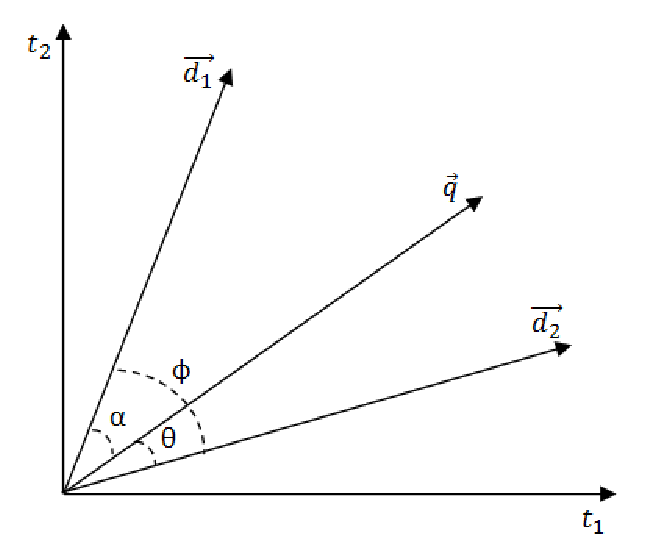
\includegraphics[scale=0.7]{img/vsm} 
	\caption[The Vector Space Model]%
           {The Vector Space Model. Documents $\vec{d_{1}}$ and $\vec{d_{2}}$, and a query vector $\vec{q}$ are represented in a two-dimensional vector space, formed by terms $t_{1}$ and $t_{2}$.}
\label{fig_vsm}
\end{figure}

A distinction has to be made between words or terms, and tokens. A term is the class which is used as a unit during parsing, and a token is each occurrence of this class. For example, in the sentence: 

\begin{quote}
\textit{CoreMedia CMS is shipped with an installation program for interactive graphical installation and configuration of the software.}
\end{quote}

the term $ installation $ is represented by two tokens. There is no universal way to parse a text, and the parsing decisions to address depend on the application in which the text collection will be used. \\

After tokenization, documents are represented as vectors, where each term is a vector in the vector space, and the documents are the sum of the terms, from which they consist. Thus, all document vectors and terms form a multi-dimensional vector space, where terms are the dimensions, and documents - the corresponding sum vectors. A diagram of the vector space is given in fig.~\ref{fig_vsm}, where two document vectors $\vec{d_{1}}$ and $\vec{d_{2}}$, and a query vector $\vec{q}$ are represented in a two-dimensional space. \\

\subsection{Weight functions}
\label{lsa:weight_functions}
Vectors in the \gls{VSM} have as elements the occurrence frequencies of words in documents. However, some documents are shorter than others, therefore one has to apply a normalization function in order to avoid representing words from longer documents as "more important" than words from shorter documents, as they would occur more often. Such normalization functions are called weight functions, and they are applied after the vector space has been constructed. \\

Weight functions are generally separated into two categories - local and global. They are often implemented as a pair together, because local functions measure the importance of a given word in a single document, while global functions give the importance of a word in the whole document collection. The most commonly used function pair is \textit{term frequency} and \textit{inverse document frequency}. \\

\subsubsection{Term frequency - inverse document frequency}
\label{lsa:tf-idf-section}
The simplest local weight is the term frequency $tf_{t,d}$. It assigns a weight to each term equal to the number of occurrences of the term $t$ in a given document $d$. However, not all words carry the same meaning in text (therefore, stop words are removed during preprocessing, as mentioned in~\ref{section_vsm}). Words that are common to all documents in the collection don't reveal much information, as compared to words which occur only in several documents. The latter are more likely to contain key information about the meaning of these documents.  This is reflected by the weight function \textit{inverse document frequency}~(eq.~\ref{lsa:idf})
\begin{equation}
\label{lsa:idf}
idf_{t}=1 + log\frac{N}{df_{t}}
\end{equation}

where $N$ is the total number of documents in the collection, $df_{t}$ is the frequency of occurrence of term $t$ in the whole collection, and $t$ is a specific term being weighted. Using $idf_{t}$ is a way to scale down the importance of commonly used words in text. When one combines both $tf$ and $idf$, a composite weight is produced for each term in each document. The \textit{tf-idf} weighting function assings to a term $t$ in a document $d$ a weight given by 
\begin{equation}
\label{lsa:tf_idf}
(tf-idf)_{t,d}=tf_{t,d} \times idf_{t}
\end{equation}. 

As defined by Manning et al.~\cite{IRbook2008}, the weight assigned to term $t$ in document $d$ by using a combination of local and global weight function is 
\begin{enumerate}
\item highest when $t$ occurs many times within a small number of documents;
\item lower when the term occurs fewer times in a document, or occurs in many documents;
\item lowest when the term occurs in virtually all documents.
\end{enumerate} 

\subsubsection{Log - entropy}
\label{lsa:log-entropy-section}
Another popular pair of weight functions, frequently used in text analysis, is the \textit{log-entropy} pair. The local function \textit{log} takes the logarithm of the raw term frequency, thus normalizing the effect when large differences in term frequencies occur. In eq.~\ref{lsa:log} $L(t,d)$ denotes the log of number of occurrence of a term $t$ in a document $d$. \\
% log
\begin{equation}
L(t,d)=\log(tf(t,d)+1)
\label{lsa:log}
\end{equation}

The global function \textit{entropy} $H(t)$ reflects the local relative importance of a term $t$ in the whole document collection~(eq.~\ref{lsa:entropy}) \\

% entropy
\begin{equation}
H(t) = 1+\frac{{\Sigma_{j}p(t,d)}}{\log n}
\label{lsa:entropy}
\end{equation}
where $n$ is the number of documents in the whole collection. In eq.~\ref{lsa:entropy}, $p(t,d)$ is defined by:
% entropy
\begin{equation}
p(t,d) = \frac{tf_{t,d}}{gf_{t}}
\end{equation}

where $gf_{t}$ is the total number of times that term $t$ occurred in all documents. The entropy measures the distribution of terms over all documents. \\

\subsection{Similarity measures}
\label{lsa:similarity_measures}
Once the vector space has been built, one can find the documents which are most similar to a given query. During \textit{query formulation}(fig.~\ref{lsa:fig:ir_process}), the queries are tokenized and represented as vectors, as already described in section~\ref{section_vsm}. Therefore, the similarities between documents and queries can be measured based on the angles between their respective vectors~(in fig.~\ref{section_vsm}, these are $ \alpha $ and $ \theta $). Using the angles between vector representations, one can define a similarity measure which is necessary for the matching process in \gls{IR} systems. The standard way to computing the similarity between two documents $d_{1}$ and $d_{2}$ is to compute the \textit{cosine similarity} of their vector representations $\overrightarrow{d_1}$ and $\overrightarrow{d_2}$ ~(eq.~\ref{lsa:cosine_measure}).

%
% cosine similarity
%
\begin{equation}
\label{lsa:cosine_measure}
sim(d1,d2)=\frac{\overrightarrow{V}(d_1).\overrightarrow{V}(d_2)}{\left\vert \overrightarrow{V}(d_1) \right\vert.\left\vert \overrightarrow{V}(d_2)\right\vert},
\end{equation}

where the numerator represents the \textit{dot product}\footnote{The dot product $\overrightarrow{x}.\overrightarrow{y}$ of two vectors is defined as $\displaystyle\sum\limits_{i=1}^{M} x_{i}y_{i} $.} of the vectors, while the denominator is the product of their \textit{Euclidean lengths}\footnote{Let $\overrightarrow{d}$ is the document vector for $d$, with $M$ components $\overrightarrow{d_{1}}...\overrightarrow{d_{M}}$. The Euclidean length of $d$ is defined to be $ \sqrt{\sum\limits_{i=1}^{M} \overrightarrow{d_{i}^2}} $}. The measure from eq.~\ref{lsa:cosine_measure} is the cosine of the angle $ \phi $ between the two vectors $\overrightarrow{d_1}$ and $\overrightarrow{d_2}$. \\

Once we represent a collection of $N$ documents as a collection of vectors, it is easy to obtain a natural view of the collection as a \textit{term-document matrix}: this is a $m \times n$ matrix whose rows represent the $m$ terms in the document collection, and each of whose $n$ columns corresponds to a document. And this specific matrix grouping all documents and terms from the collection is used in \textit{Latent Semantic Analysis}, a technique which is discussed next.\\

\section{Latent Semantic Analysis}
\gls{LSA} was first introduced by Dumais et al.~\cite{Dumais88usingLSA} and Deerwester et al.~\cite{Deerw90_LSA} as a technique for improving information retrieval. It is based on the Vector Space Model, where as already discussed, words from users' queries are matched with the words in documents. Such \gls{IR} models that depend on lexical matching have to deal with two problems: \textit{synonymy} and \textit{polysemy}. Due to the many meanings which the same word can have, also called polysemy, irrelevant information is retrieved when searching. And as there are different ways to describe the same concept, or synonymy, important information can be missed. \gls{LSA} has been proposed to address these fundamental retrieval problems, having as a key idea dimension reduction technique, which maps documents and terms into a lower dimensional semantic space. \gls{LSA} models the relationships among documents based on their constituent words, and the relationships between words based on their occurrence in documents. By using fewer dimensions than there are unique words, \gls{LSA} induces similarities among words including ones that have never occurred together~\cite{Dumais2006}. The basic steps in using \gls{LSA} are: document representation (the same as in \gls{VSM}), \gls{SVD} with dimensionality reduction, and querying. Next, the theoretical basis for \gls{LSA} is given, as it has been implemented as a part of this work. \\


As mentioned above, the first step of \gls{LSA} implementation is document representation. It is similar to the representation in \gls{VSM}, therefore refer to section~\ref{sec:lsa:doc_repres}. After tokenizing all documents in the collection, and computing the corresponding term weights, one has to construct a term-document matrix~(eq.~\ref{lsa:sparse_matrix_A}). Having as rows the terms, and as columns the documents, its elements are the occurrences of each term in a particular document, where $ a_{ij} $ denotes the frequency with which term $ i $ occurs in document $ j $. The size of the matrix is \text{\bf{m x n}}, where {\bf m} is the number of terms, and {\bf n} is the number of documents in the text collection. Since every term doesn't appear in each document, the matrix is usually sparse. \\

%
% initial sparse matrix A
%
\begin{equation}
A=
\begin{bmatrix}
\label{lsa:sparse_matrix_A}
 a_{11}& a_{12}& \cdots& a_{1n} \\
 \vdots& \vdots& \ddots& \vdots \\ 
 a_{m1}& a_{m2}& \cdots& a_{mn}
\end{bmatrix}
\end{equation}\\

Local and global weightings are applied to increase or decrease the importance of terms within documents. After presenting the most popular weight functions in sections~\ref{lsa:weight_functions}, we can write
%
% general weighting function
%
\begin{equation}
\label{lsa:global_local_weighting}
a_{ij}=L(i,j) \times G(i),
\end{equation}

where $L(i,j)$ is the local weighting of the term $i$ in document $j$, and $G(i)$ is the global weighting for term $i$. As examples of local functions, the term frequency $tf$ and $log$ were discussed, while $idf$ and entropy were the examples for global weightings. The choice of weight function impacts \gls{LSA} performance. In section~\ref{sec:lsa:factors_infl_lsa} reasons are given for the specific implementation decisions made in this work concerning \gls{LSA}. \\

\section{Singular Value Decomposition}
\label{sec:lsa:svd}

After its generation, the term-document matrix is decomposed into three matrices~(eq.~\ref{lsa:svd}) by applying \gls{SVD}. It is a unique decomposition of a matrix into the product of three matrices - $U$, $V$ and $\Sigma$, where $U$ and $V$ are orthonormal matrices\footnote{An orthonormal matrix is a matrix, whose columns, treated as 
 vectors, are also orthonormal. A matrix is orthonormal, if its transpose is equal to its inverse. For more information on matrices and matrix operations, refer to~\cite{MatrixCompGolub96}}, and $ \Sigma $ is a diagonal matrix\footnote{A diagonal matrix is a square matrix, in which the entries outside the main diagonal are all $0$.} having singular values\footnote{For a square matrix $A$, the square roots of the eigenvalues of $A^{T}A$, where $A^{T}$ is the conjugate transpose, are called \textit{singular values}. Given a matrix $A$, a non-zero vector $x$ is defined to be an \textit{eigenvector} of the matrix, if it satisfies the \textit{eigenvalue equation}: $Ax=\lambda x$ for some scalar $ \lambda $. The scalar $ \lambda $ is called an \textit{eigenvalue} of $A$ corresponding to the eigenvector $x$.\cite{MatrixCompGolub96}} on its diagonal.\\
%
% SVD decomposition in three matrices
%
\begin{equation}
\label{lsa:svd}
A=U \Sigma V^{T}
\end{equation}

After the initial matrix $A$ is decomposed, all but the highest $k$ values of its product diagonal matrix $\Sigma$ are set to $0$. When $A$ is recomputed again following eq.~\ref{lsa:svd}, the resulting  matrix $A_{k}$ represents the semantic space of the text collection. A classical visual example can be used to presenting \gls{SVD}~(as given in \cite{Dumais88usingLSA}) into three product matrices. It can be seen here how the dimensionality reduction of matrix $\Sigma$ affects all three product matrices.\\
%
% diagram of the truncated SVD
%
\begin{center}
\begin{figure}[htbp]
	\centering
	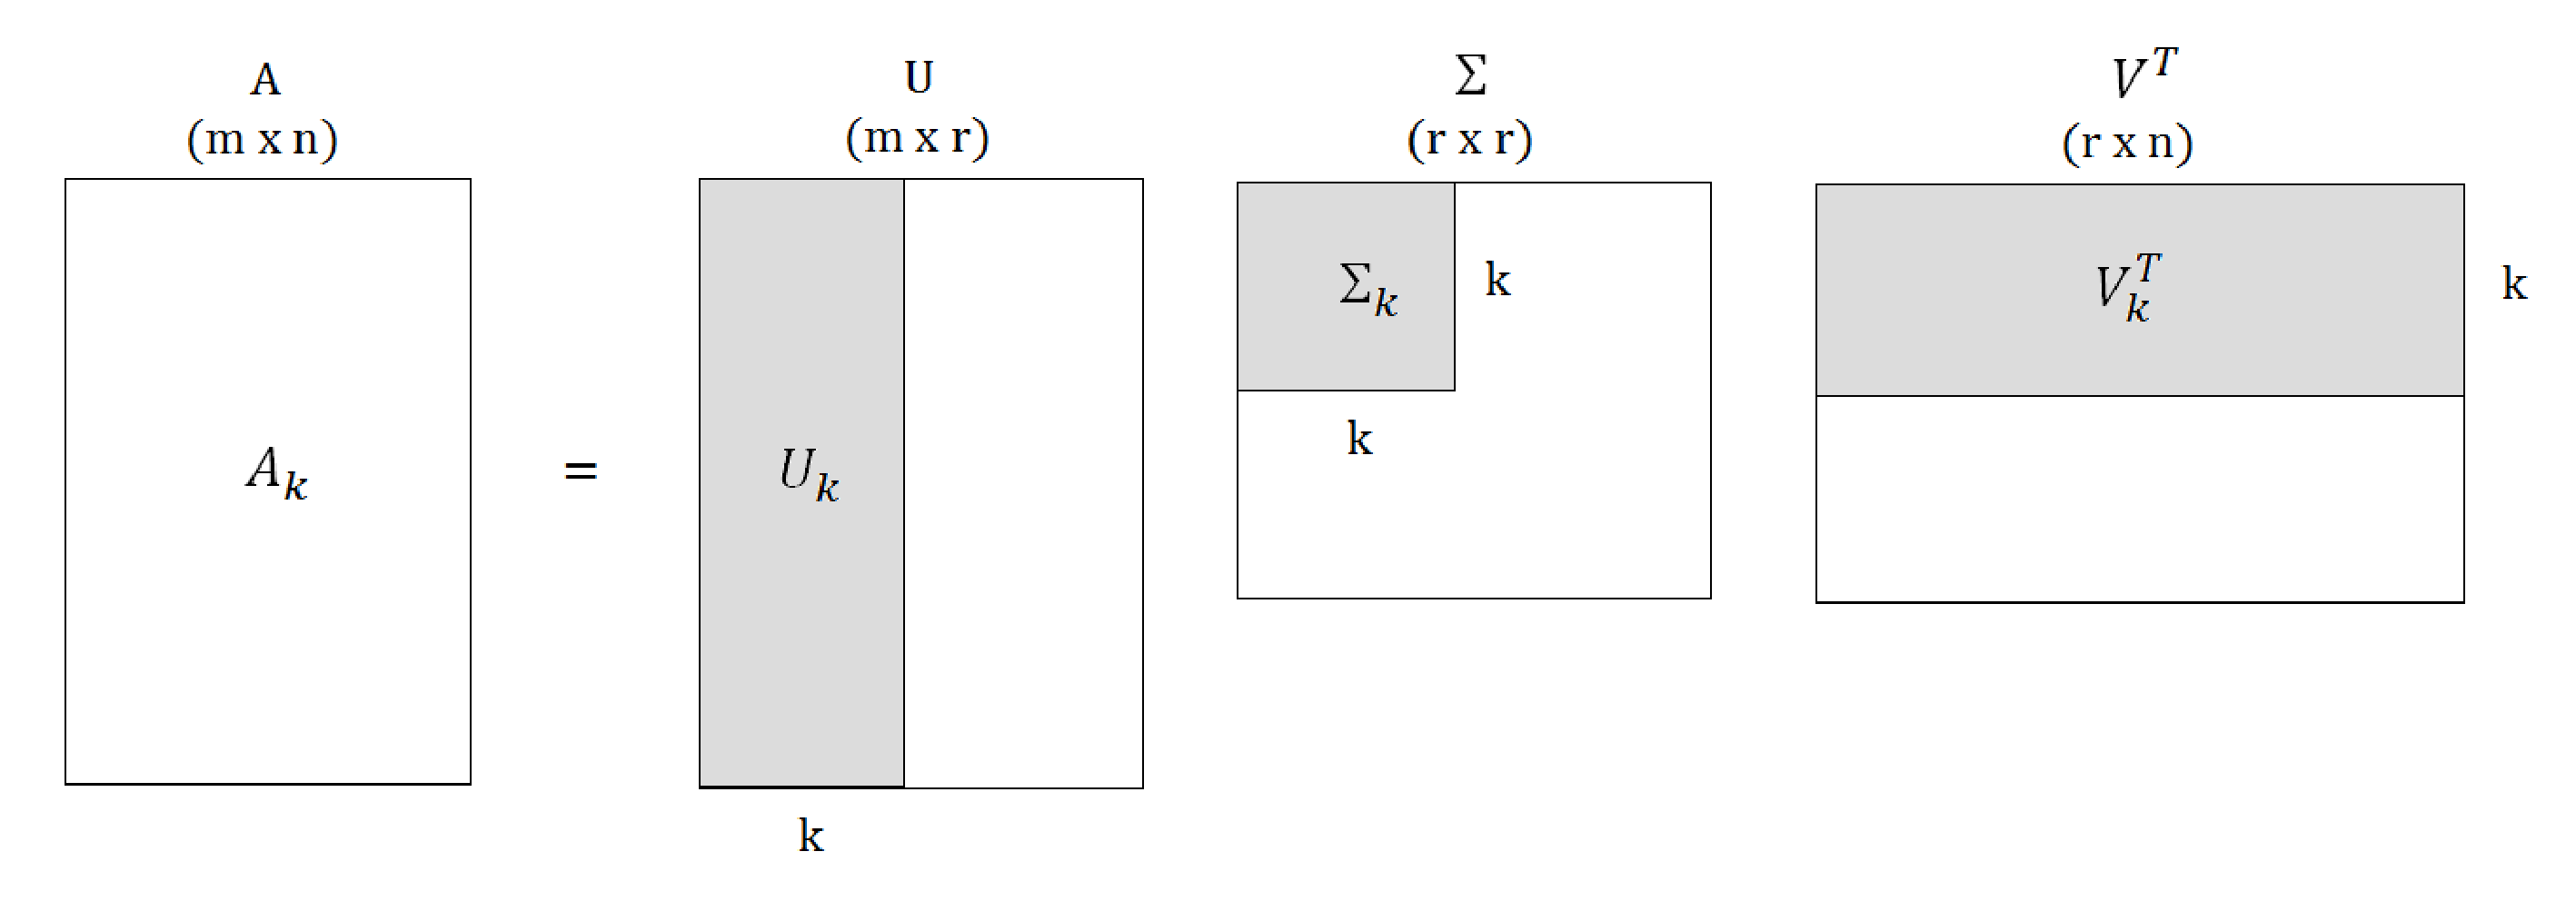
\includegraphics[width=\ScaleIfNeeded]{img/svd} 
 % or [scale=0.5]
	\caption[Diagram of truncated SVD]%
           {Diagram of truncated SVD}
\label{lsa:truncated_svd}
\end{figure}
%
% description of the parameters in SVD diagram
%
\begin{tabular}{l l}
$A_{k}$ - best rank-$k$ approximation of $A$ & $m$ - number of terms\\
$U$ - term vectors & $n$ - number of documents \\
$\Sigma$ - singular values & $k$ - number of factors \\
$V^{T}$ - document vectors & $r$ - rank of $A$ \\
\end{tabular}
\end{center} 

In fig.~\ref{lsa:truncated_svd}, $U$ and $V$ contain the term and document vectors respectively, and $\Sigma$ is constructed by the singular values of $A$. An important property of \gls{SVD} is that the singular values placed on the diagonal of $\Sigma$ are in decreasing order. Hence, if all but the first $k$ singular values are set to $0$, the semantic meaning in the resulting space is preserved to some approximation $k$, while noise or variability in word usage, is filtered out. Noise in this case are the terms with lowest weights which carry little meaning. By using fewer dimensions $k$, \gls{LSA} induces similarities among terms including ones that have never occurred together. Terms which occur in similar documents, for example, will be near each other in the k-dimensional vector space even if they never co-occur in the same document. This means that some documents that do not have any common words with a given query may be near it in resulting k-space.\\

A factor to be considered when computing \gls{SVD} is the run-time complexity of the algorithm. For decomposition of very large matrices, it is $O(n^2k^3)$, where $n$ is the number of terms in the text corpus, and $k$ is the number of dimensions in semantic space after dimensionality reduction. Note that  $k$ is typically a small number between 50 and 350.\\

A more detailed description of \gls{SVD} can be found in \cite{Berry95usinglinear} and \cite{MatrixCompGolub96}.\\

\section{Querying the semantic space}
\label{lsa:querying_sspace}

In this work \gls{LSA} is used for \gls{IR} purpose. Therefore, the final step of applying the technique is to pose queries on the constructed semantic space. A query $q$ is a set of words which must be represented as a document in the k-dimensional space, in order to be compared to other documents. The user's query can be represented by using eq.~\ref{lsa:query}:
%
% Query translation for LSA
%
\begin{equation}
\label{lsa:query}
q = q^{T}U_{k}\Sigma_{k}^{-1}
\end{equation}\\
where $q$ is the set of words in the query, multiplied by the reduced term and singular values matrices. Using the transformation in~eq.~(\ref{lsa:query}), the query is ''mapped'' onto the reduced k-space. After the mapping, the resulting query vector can be compared to the documents in the k-space, and the results ranked by their similarity or nearness to the query. A common similarity measure used to compute similarity between the query and the document vectors is the cosine~(eq.~\ref{lsa:cosine_measure}). From the resulting document set, the documents closest to the query above certain threshold are returned as search results. \\

\section{Factors which influence LSA performance}
\label{sec:lsa:factors_infl_lsa}
The effective usage of \gls{LSA} is a process of sophisticated tuning. Several factors can influence the performance of the technique. These factors are pre-processing of texts~(removal of stop-words, filtering, stemming), frequency matrix transformations, choice of dimensionality $k$, choice of similarity measure. Dumais et al.~\cite{dumais91improving} and Nakov et al.~\cite{Nakov_weightfunctions} have carried out research on \gls{LSA} performance depending on the choice of the above mentioned factors. They conclude that \gls{LSA} performance depends on the particular text corpus, as well as on the purpose of \gls{LSA} application. However, in the case of matrix transform, log-entropy~(section~\ref{lsa:log-entropy-section}) performs better as compared to other matrix transform function combinations, including the popular term frequency - inverse document frequency~($tf-idf$)~(section~\ref{lsa:tf-idf-section}). Therefore, the former is implemented in this work. It has been further stated~(\cite{dumais91improving},\cite{NakovBetterResultsLSI}) that with respect to similarity measures used, \gls{LSA} performs optimal when cosine similarity measure is implemented to calculate the distance between vectors in the semantic space~(eq.~\ref{lsa:cosine_measure}). It is therefore used in this work to measure the relevance between queries and documents. And finally, the dimensionality reduction parameter $k$ is defined empirically based on the experimentation results presented in Chapter~\ref{chapter:evaluation}.

\chapter{Cluster labeling}
A major problem in text analysis is to determine the topics in a text collection and identify the most important or significant relationships between them. Clustering and visualizations (tag clouds) are key analysis methods in order to address this problem. In this chapter, we discuss three algorithms for cluster labeling, which are relatively new, and in Chapter~\ref{sec:tagclouds} we introduce tag clouds as a visualization mean used in \gls{IR} systems. \\

\section{Clustering}
\textit{Clustering} is an \gls{IR} method that groups objects (documents) together based on their similarities in so called clusters. Such methods are often applied in the post processing phase of \gls{IR}~(fig.~\ref{fig:text_analysis}) for visualization of retrieved results. For example, similar search results can be grouped together during presentation of results in search engines. \\

Clustering can be used for categorization of resources (documents). \textit{Document categorization} is the process of assigning a document to one or more categories. A categorization $C = \{c_{1}, c_{2}, ..., c_{k}\}$ partitions a document collection $D$ into subsets $c \subseteq D$, so that $ \cup_{i=1}^{k} c_{k} =D $. $C$ is exclusive categorization if $c_{i} \cap c_{j \ne i} = 0, c_{i}, c_{j} \in C$, and non-exclusive categorization otherwise. Clustering is an \textit{unsupervised categorization method}, as it organizes documents into clusters without having prior knowledge about the clusters, or predefined cluster categories.\\
 

Presenting search results in groups, or categories, should help users gain a quick overview of the retrieved documents. An important part of clustering used for visualization of results, is choosing choose suitable labels of the categories defined, so that they are usable to human users. The process of \textit{cluster labeling} creates labels for clustered groups of objects. \\

\subsection{Clustering algorithms}
\label{sec:clustering_algorithms}
A large variety of clustering algorithms exists, and they are usually classified according to the characteristic of their output structure. Jain et al.~\cite{clusteringJain99} make a classification based on the following properties: \\

\textbf{Flat vs. hierarchical clustering} \\
\textit{Flat clustering} creates a flat set of clusters without relations between clusters due to some structure. K-means is a popular clustering algorithm, which creates as output a flat structure of document clusters. We present K-means clustering algorithm as an example for flat clustering in section~\ref{clustering:algo}. \textit{Hierarchical clustering} on the other hand creates a hierarchy of clusters, with parents and children, in a tree-like manner. ?citation needed for hac definition?\\

\textbf{Hard vs. soft clustering}\\
Another important distinction can be made between \textit{hard} and \textit{soft} (also called fuzzy) clustering algorithms. If each document is assigned to a single cluster only, we have hard clustering. Otherwise, clustering is soft, and it assigns a document as a distribution over all clusters. This means that each document can have a fractional membership in several clusters. \gls{LSA}~(Chapter~\ref{sec:lsa}) is a good example for a soft clustering algorithm. K-means is a popular example for hard clustering~(section~\ref{clustering:algo}). \\


\textbf{Monothetic vs. polythetic clustering} \\
Based on how documents are assigned to different clusters, clustering can be divided into \textit{monothetic} and \textit{polythetic}~\cite{hierarchMonotheticClustering2004}. Monothetic algorithms assign a document to a cluster based on a single feature, while polythetic algorithms classify documents by overall degree of similarity/difference calculated over many properties. This makes monothetic clustering well suited for generating hierarchies and browsing search results, since a single feature, common to all documents in the cluster, describe each cluster. Users understand easily clusters generated in this way. K-means is an example of polythetic document clustering algorithm, where each cluster is described by several words of phrases. \\



\subsection{K-means clustering algorithm}
\label{clustering:algo}
In this work we use K-means algorithm in order to cluster documents, which we need for the evaluation of cluster labeling algorithm~\gls{WCC}. Two factors influence this implementation decision:
\begin{itemize}
\item As we use \gls{LSA} to process the term-document matrix, we can investigate which dimensionality reduction parameter $k$ is optimal for our case, so that we can obtain the optimal number of topics (or soft clusters) for our evaluation data set. Therefore, we should not suffer from one of k-means's weaknesses, namely having to define as initial parameter the number of clusters, since we use as a cluster number the dimensionality reduction parameter, previously defined in \gls{LSA}.
\item Another reason to use k-means algorithm is its simplicity, as compared for example to \gls{HAC} - the complexity of k-means is linear, while the complexity of \gls{HAC} is exponential. \\
\end{itemize}

\textit{K-means} is an example for flat, hard and polythetic clustering algorithm, based on the classification mentioned previously. It was first introduced by Lloyd~\cite{kmeans_Lloyd82}. The algorithm outputs a flat unstructured set of clusters. It starts by dividing the document collection into $k$ clusters, where $k$ is an input parameter, and then computes the $k$ \textit{means} of these clusters. K-means defines a cluster in terms of a \textit{centroid}, usually the \textit{mean of a group of points}, and is applied to objects (documents) in n-dimensional space (such as vector space). After the initialization, the following two steps are iteratively repeated, until the clusters are not re-assigned any more: \\
\begin{enumerate}
\item Each document in the collection is assigned to the cluster with the closest mean.
\item For each cluster, new means are recomputed based on the documents it contains.
\end{enumerate}

In algorithm~\ref{algorithm_kmeans} we give as pseudo-code a detailed step-by-step description of k-means algorithm. \\


\renewcommand{\algorithmicrequire}{\textbf{Input:}}
\renewcommand{\algorithmicensure}{\textbf{Output:}}
\begin{algorithm}
\caption{K-means clustering algorithm}
\label{algorithm_kmeans}
\begin{algorithmic}
\REQUIRE $D = \{d_{1}, d_{2}, ..., d_{n}\}$ - documents to be clustered \\
         $k$ - number of clusters \\
\ENSURE $C = \{c_{1}, c_{2}, ..., c_{k} \}$ - clusters \\
        $ m : D \rightarrow \{1 ... k \} $ - cluster membership \\
\STATE Set $C$ to initial value (e.g. select $k$ random points as initial centroids) \\
\COMMENT{Form $k$ clusters by assigning each document to its closest centroid}
\FORALL{$d_{i} \in D$}
\STATE $m(d_{i}) = mindistance_{j \in \{1..n \}}(d_{i}, c_{j})$
\ENDFOR \\
\COMMENT{Recompute the centroid of each cluster until centroids do not change}\\
\WHILE{$m$ has changed}
\FORALL{$ i \in \{1..n \}$}
\STATE Recompute $c_{i}$ as the centroid of $ \{d | m(d) = i \} $
\ENDFOR
\FORALL{$d_{i} \in D$}
\STATE $m(d_{i}) = mindistance_{j \in \{1..n \}}(d_{i}, c_{j})$
\ENDFOR
\ENDWHILE
\end{algorithmic}
\end{algorithm}

\textbf{TODO}: Give + and - of this method. \\

\section{Cluster labeling}
\label{sec:cluster_labeling}
Assume that a categorization over a document collection is determined using an unsupervised approach (e.g. clustering). To present this categorization to a user, it is convenient to label the individual categories with characteristic terms. These terms, called \textit{category labels}, should characterize the content of the associated category with respect to the remaining categories. This implies that cluster labeling should \textit{summarize} a category's content and that it should \textit{discriminate} a category from the other categories. This section states desired properties of category labels and presents an algorithm which generates such labels. It further makes a proposition for improvement of \gls{WCC}~(section~\ref{clustering:WCC}) algorithm, and in Chapter~\ref{sec:implementation} offers an evaluation of \gls{WCC}, using k-means clustering. \\

\subsection{Clustering and labeling}
In their paper from 2009~\cite{surveyWebClusteringEngines2009}, Carpineto et al. claimed that there is a difference between clustering of data sets, and clustering of search results, returned from search engines:~\textit{"in search results clustering description comes first"}. Thus, in contrast to the classical categorization of clustering algorithms we previously outlined, they proposed a classification based on how well the clustering algorithms can generate sensible, comprehensive and compact cluster labels, and divided algorithms in the following three categories: \\

\textbf{Data-centric algorithms} \\
Data-centric algorithms were the first ones to be implemented for cluster labeling. Here, clustering is done with some general clustering algorithm, and terms which are close to the cluster centroids are nominated as cluster labels. Cluster centroids are a collection of independent terms from all documents not related to each other. In order to define the terms from cluster centroid, one uses a frequency measure, such as $tf-idf$~(eq.~\ref{lsa:tf_idf}). We present \gls{WCC}~(see~\ref{clustering:WCC}) as an example for a data-centric clustering algorithm. \\

\textbf{Description-aware algorithms} \\
While data-centric algorithms don't consider word order, and process documents as "a bag of words", description-aware algorithms process ordered sequence of words (phrases), instead of terms, as candidate labels, and assign labels during clustering process, not after it. Using monothetic term selection, one nominates frequent phrases containing a noun head as labels, which are interpretable to human users. Clustering and labeling are closely related, and labeling influences the clustering process. Therefore, it is not possible to combine the labeling with any clustering algorithm. \gls{STC} is an example of a description-aware algorithm, introduced by Zamir and Etzioni~\cite{suffixTreeClustering99}. \gls{STC} builds a tree from the most frequent phrases in documents by using the data structure \textit{suffix tree}~\cite{suffixTreeClustering99}. It group documents that have common phrases under the same nodes of the tree. Thus, all documents below a given node contain the phrase at the node. \\

\textbf{Description-centric algorithms} \\
These algorithms operate on the principle \textit{"description comes first"}, and in this sense are the opposite of the data-centric algorithms. The goal here is to find meaningful cluster labels. If there are no suitable labels found, the cluster has no value for the users (doesn't have a proper visualization), and is therefore discarded. Description-centric algorithms are mainly applied for clustering of search results~(more information can be found in~\cite{surveyWebClusteringEngines2009}). \\

\subsection{Formal framework for cluster labeling algorithms}
When we use an unsupervised approach to categorize a collection of documents, such as clustering, we also need to label the categories defined, in order to present them to users. The category labels should characterize the given categories - labels should summarize category content, and should discriminate a category from other categories~\cite{Stein04topicidentification}. Until now, no uniformly agreed upon formal framework exists that defines the requirements for cluster labeling algorithms. There are publications which name desired properties for cluster labels (\cite{formal_cluster_labels2003},~\cite{dweiss2006} ), but they all give informal descriptions. Stein and Meyer Zu Eissen~\cite{Stein04topicidentification} have given their definitions for desired properties of cluster labeling algorithms as a formal framework. We base our definition below on this source. \\

If we have an unstructured collection of documents $D$, a clustering algorithm creates a categorization for this collection in the form $ C = \{ c_{1}, c_{2}, ..., c_{k} \} $, where the sets $c_{i}$ are subsets of $D$, and their union covers $D$: $\cup_{c_{i}\in C} c_{i} = D$. When applying a hierarchical clustering algorithm, this implies a cluster labeling hierarchy $H_{C}$ over $C$. Then, $H_{C}$ is a tree and its nodes are the categories in $C$, having one node as a root. Let $c_{i}, c_{j} \in C, c_{i} \ne c_{j}$ are two categories. If $c_{j}$ is a child cluster of $c_{i}$, then $c_{i}$ is closer to the root of the hierarchy $H_{C}$, and we write $c_{i} \succ c_{j}$. \\

For an existing categorization $C$, we therefore need a cluster labeling $ \text{\L} = \{ l_{1}, l_{2}, ..., l_{k} \} $. \\


Let $T = \cup_{d \in D}T_{d} $ is the term set in the given document collection $D$. As defined by Stein and Meyer zu Eissen~\cite{Stein04topicidentification}, a cluster labeling function $ \tau : c \shortrightarrow \text{\L} $ assigns a cluster label to each cluster $ c \in C $, where $\text{\L}_{c} \subset T$. \\


Thus, the following properties are desired for a cluster labeling function: \\
\begin{enumerate}
\item \textbf{Unique} \\
Cluster labels should be unique. The same terms should not be assigned as cluster labels to more than one cluster, or no two labels should include the same terms from two different clusters. \\
\begin{equation}
\forall_{
\substack{ c_{i},c_{j} \in C, \\ c_{i}\neq c_{j}}
} : \tau(C_{i}) \cap \tau(C_{j}) = 0
\end{equation}

 
\item \textbf{Summarizing} \\
If possible, the label of a cluster $c$ should contain at least one term $t$ from each document $ d\in c$. Terms occurring in all documents, which are part of the cluster, represent it better than terms that occur only in few documents. \\
\begin{equation}
\forall_{ c \in C}, \forall_{ d \in c} : \tau{c} \cap T_{d} \neq 0
\end{equation}
where $T_{d}$ is the set of terms in document $d$.

\item \textbf{Discriminating} \\
Apart from summarizing, terms in labels should be discriminating. They should contribute to discriminate the cluster from other clusters, i.e. the same terms should be present in a considerably smaller set of documents in the other clusters. In cluster label $c$ exists a term $t$ whose frequency of occurrence is relatively higher in the documents of the cluster as compared to other clusters. \\
\begin{equation}
\forall_{
\substack{ c_{i},c_{j} \in C \\ c_{i}\neq c_{j}}}
 \exists_{ t \in T{c_{i}}} : \frac{tf_{c_{i}}(t)}{\left| c_{i} \right|} \ll \frac{tf_{c_{i}}(t)}{\left| c_{j} \right|}
\end{equation}
Here, $T_{c_{i}}$ is the term set in category $c_{i}$, and $tf_{c_{i}} (t)$ is the term frequency of term $t$ in category $c_{i}$, or the sum of $tf (t)$ in all documents in cluster $c_{i}$ : $tf_{c_{i}} (t) = \sum_{d \in c_{i}}{tf_{d} (t)} $. \\


\item \textbf{Expressive} \\
Terms forming a label of cluster $c$ should have highest frequency of occurrence in the documents from $c$:
\begin{equation}
\forall_{c \in C} \forall_{d \in c} \forall_{t \in T_{d}} : tf_{d}(t) \leq tf_{d}(t'), t' \in \tau(c)
\end{equation}
Here, $tf_{d}(t)$ is the term frequency of occurrence of term $t$ in document $d$.

\item \textbf{Contiguous} \\
This property holds for consecutive terms, for example belonging to a phrase. Such cluster labels, containing consecutive terms, are more understandable to human users.
\begin{equation}
\forall_{c \in C} \forall_{
\substack{t, t' \in \tau(c), \\ c_{i} \ne c_{j}}
} \forall_{d \in c} \exists_{t_{i}, t_{i+1} \in T_{d}} : t_{i} = t \wedge t_{i+1} = t'
\end{equation}

\item \textbf{Hierarchically consistent}
\begin{equation}
\forall_{
\substack {c_{i}, c_{j} \in C, \\ c_{i} \ne c_{j}}
} : c_{i} \succ c_{j} \Rightarrow P(t_{i} | t_{j}) = 1 \wedge P(t_{j} | t_{i}) < 1,
\end{equation}
where $t_{i} \in \tau(c_{i})$ and $ t_{j} \in \tau(c_{j}) $. This property is required only when using a hierarchical clustering algorithm (e.g. \gls{STC}~\cite{suffixTreeClustering99}).

\item \textbf{Irredundant} \\
Irredundancy complements the property \textit{unique}. Terms which are synonyms should be avoided in cluster labels. \\
\begin{equation}
\forall_{ c \in C}, \forall_{
\substack{t,t' \in \tau{c}, \\ t \ne t'}
} : \mbox{ t and t' are not synonyms }
\end{equation}

\end{enumerate}

The properties stated above describe ideal conditions and can only be approximated in the real world. One needs external knowledge (e.g. an ontology), in order to fulfill properties \textit{hierarchical consistency} and \textit{irredundancy}. \\

\subsection{Weighted Centroid Covering}
\label{clustering:WCC}
Weighted Centroid Covering was introduced by Stein and Meyer zu Eissen~\cite{Stein04topicidentification}. It is a data-centric algorithm for cluster labeling, in which labels are generated from sets of frequently occurring terms. \\

If $D$ are all documents in a collection, which contains a set of terms $T$, and $t \in T$ is a term from $T$, and $C = \{c_{1}, c_{2}, ..., c_{\left| C \right|} \}$ is a categorization over the set $D$, then we can define a function $\kappa$ as follows:
let $\kappa : T \times \{c_{1}, c_{2}, ..., c_{\left| C \right|} \} \rightarrow C$ is a function with $\kappa(t,i) = c$ iff $c$ is the cluster with $i$th frequent occurence of term $t$~\cite{Stein04topicidentification}. As an exaple, if $t$ occurs most frequently in a give cluster, we can write $\kappa(t,1)$, and if it occurs least frequently, we write $\kappa(t,\left|C\right|)$. \\

% wcc graphically presented simplified
\begin{figure}[H]
\centering
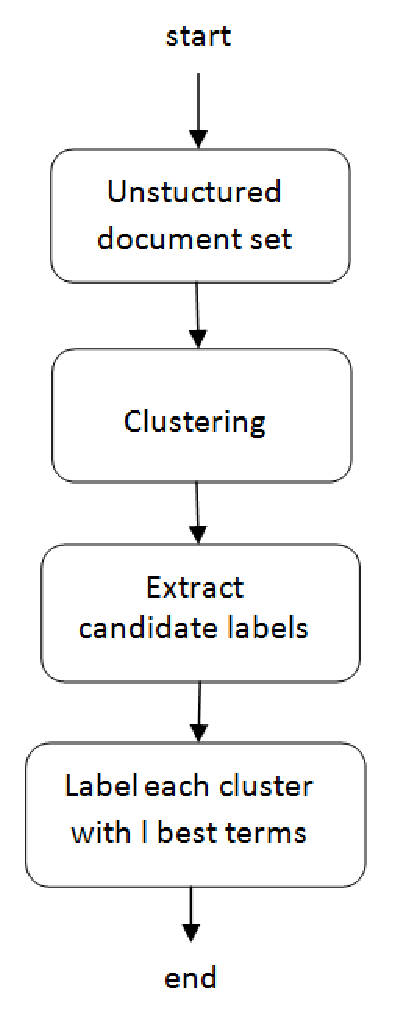
\includegraphics[scale=0.6]{img/wcc}
\caption[Cluster labeling using WCC]%
           {Cluster labeling using Weighted Centroid Covering algorithm}
\label{fig_wcc}
\end{figure}

\gls{WCC} algorithm consists of three stages. As input to the algorithm, we input a clustering $C$:
\begin{enumerate}
\item For all terms in the input clusters, it saves the $k$ most frequent occurrences of each word with its term frequency, and the cluster in which it occurs, to a data structure (say a vector \L).
\item It sorts vector \text{\L} ~which stores tuples ($k$, $tf(term)$, term, cluster) in a descending order, based on the frequency of a term in a given cluster $tf_{c}(t)$;
\item It assigns $l$ number of terms to each cluster as labels. Therefore, in the end each cluster has a label of $l$ terms, assigned to it in a Round-Robin-like manner. \\
\end{enumerate}

The complexity of \gls{WCC} is $O(\left| T\right . log(\left|T \right|))$. A pseudo code of the algorithm is given as algorithm~\ref{algorithm_wcc}. Additionally, the main steps of \gls{WCC} can be seen graphically in fig.~\ref{fig_wcc}.\\

%\floatname{algorithm}{Procedure}
\renewcommand{\algorithmicrequire}{\textbf{Input:}}
\renewcommand{\algorithmicensure}{\textbf{Output:}}
\begin{algorithm}
\caption{Weighted Centroid Covering algorithm for cluster labeling}
\label{algorithm_wcc}
\begin{algorithmic}
\REQUIRE $C$ - clustering \\
         $l$ - number of terms per label \\
         $k$ - maximum occurrence of the same term in different labels
\ENSURE $\tau$ - labeling function
\STATE $\text{\L} = 0$
\STATE \textbf{foreach} $c$ in $C$ \textbf{do}
\STATE $\tau(c) = 0; $
\STATE \textbf{end foreach}
\STATE \textbf{foreach} $t$ in $T$ \textbf{do}
\FOR{$i = 1$ to $k$}
\STATE compute $c = \kappa(t,i)$ from $C;$
\STATE add tuple $ \langle t, tf_{c}(t)\rangle$ to $\text{\L};$
\ENDFOR
\STATE \textbf{end foreach}
\STATE \textbf{sort} $\text{\L} $ according to descending term frequencies;
\FOR{$labelcount = 1$ to $l$}
\STATE $assigned = 0;$
\STATE $j = 1;$
\WHILE{$assigned < \left|C\right|$ \AND $j \le \left|\text{\L}\right| $}
\STATE let $t_{j} = \langle t, tf_{c} (t)\rangle$ be $j^{th}$ tuple of \text{\L};
\IF{$\left|\tau(c)\right| < labelcount$}
\STATE $\tau(c) = \tau(c) \cup \{t\}$;
\STATE delete $t_{j}$ from $ \text{\L} ;$
\STATE $assigned = assiged + 1;$
\ENDIF
\STATE $j = j + 1;$
\ENDWHILE
\ENDFOR
\STATE \textbf{foreach} $c$ in $C$ \textbf{do}
\STATE \textbf{do} sort $\tau(c)$
\STATE \textbf{end foreach}
\RETURN $\tau;$
\end{algorithmic}
\end{algorithm}



\section{Cluster labeling using external knowledge}
We previously presented WCC as an algorithm for cluster labeling. It nominates cluster labels by selecting as candidate labels the terms with highest frequency of occurrence from the corresponding clusters. In order to improve labeling for users, we may consider using noun phrases for labels, as they are intuitively understood by humans, and are more descriptive than single terms. In order to improve labeling, we propose using an ontology as an external knowledge for the cluster labeling algorithm, and to nominate candidate labels from both ontology and most frequently occurring terms in clusters. Thus, if ontology fails to provide suitable labels, we can fall back to the label candidates proposed by WCC. \\

In order to present our approach, first we give a short overview on ontologies. As it is not the topic of this work to investigate into semantic knowledge and ontologies, in order to gain more detailed insight, refer to the given reference literature. 

\subsection{Ontology as a source of external knowledge}
Formal models of the world can be used to provide formal semantics, or machine-interpretable meaning to information, stored as documents, web pages, databases. When models are intended to represent a shared conceptualization, such as classification, they are called ontologies~\cite{SemSearch_IRmodels09}. Or if we use a classical definition from Gruber~\cite{ontology2005}: �Ontologies are specifications of the conceptualizations at a semantic level.� \\

Formal ontologies are represented in logical formalism which allows for indexing, querying, and reference purposes over non-ontological datasets, such as documents, databases [23]. An example for a logical formalism is the ontology language \gls{OWL}\footnote{{http://www.w3.org/TR/owl-features/}, accessed December, 2010}. \\

An ontology is characterized by the following tuple (ordered list): \\
\begin{eqnarray}
O = <C, R, I, A>
\end{eqnarray}

In the equation above $C$ is a set of classes which represent the concepts from a given domain. Examples for concepts can be databases, resources, repositories. $R$ is a set of relations, also called properties or predicates. These relations are valid between instances of the classes from $C$. As an example: Resource \textit{isStoredIn} Repository. $I$ is a set of instances, having as elements instances to one or more classes, which can also be linked to other instances or values. For example: \textit{manual2} isStoredIn \textit{onlineRepository1}. And finally, $A$ is a set of axioms, or rules, such as for example (TODO: give a meaningful example for an axiom). \\

According to the formal language used for their creation, ontologies can be divided into \textit{lightweight} and \textit{heavyweight}. Heavyweight ontologies possess highly predictive and restrictive concept definitions; as compared to them, lightweight ontologies allow for more efficient and scalable reasoning [23]. Based on the conceptualization that they describe, the ontologies can be divided further into \textit{upper-level}, which model general knowledge and \textit{domain} ontologies, specific to a certain domain (e.g. the domain of CoreMedia \gls{CMS}).

\subsection{TODO: Weighted Centroid Covering augmented by an ontology}
Stein and Meyer zu Eissen~\cite{Stein04topicidentification} point out that this \gls{WCC} could be extended to use existing ontologies and labels, but they provide no experimental results of any kind. \\

Cluster labeling by using \gls{WCC} has certain limitations. It has been suggested~(\cite{Stein04topicidentification}) to use external knowledge during cluster labeling generation, such as an ontology. Other sources~(\cite{cluster_labeling_wiki_2009}) propose using Wikipedia in order to collect candidate labels for the clusters previously created.\\

- a collection of cluster label candidates can be prepared a priori (an ontology) and
reused with no additional computational cost. \\

- candidate labels can come from a different source - a predefined ontology (to guarantee they are comprehensible). Thus, cluster label comprehensibility and cluster descriptions can be improved by using data extracted from a predefined ontology\\

We propose using external knowledge during extraction of candidate la-
bels phase (fig.~\ref{fig_wcc_onto}). \\

% wcc with ontology
\begin{figure}
\centering
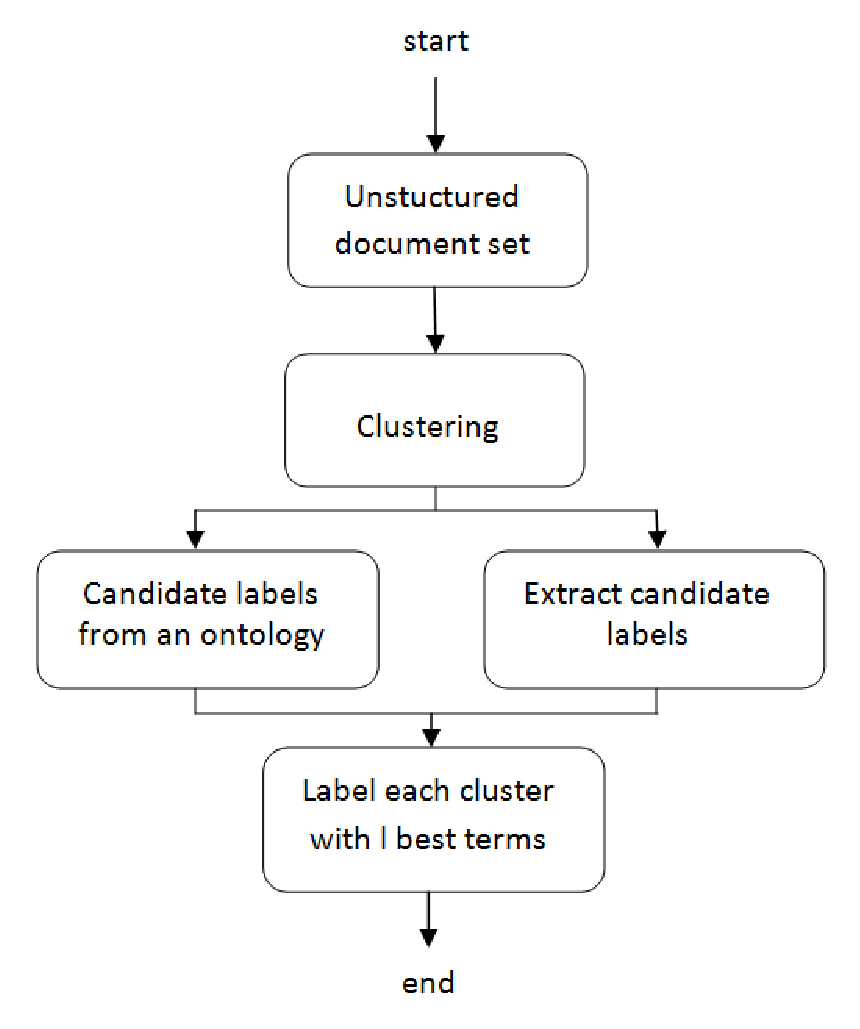
\includegraphics[scale=0.6]{img/wcc-onto}
\caption[Cluster labeling using WCC with external knowledge]%
           {Cluster labeling using Weighted Centroid Covering algorithm, augmented by an ontology}
\label{fig_wcc_onto}
\end{figure}



candidate labels are extracted from an ontology in addition to the important terms that are extracted directly from the cluster content. Thus, selected ontological categories "compete" with inner terms for serving as the cluster labels. In general, prepared ontological categories are a successful resource for labeling; however, inner terms should be considered for the cases when the ontology fails to cover the cluster content. \\

%The best scenario is that cluster labels should present a conceptualization of the documents in text corpus. This is not achieved by the algorithm presented. Technically, a hierarchical clustering algorithm can construct from each Document set $D$ a category tree. However, the labeling based on this hierarchical clustering will be far from a semantical taxonomy. This weakness of the algorithm presented can be corrected by using an external classification knowledge, e.g. an upper-level ontology. \\

%Unfortunately, domain ontologies usually have coverage limitations because not all the terms of the domain are included in the ontology.\\

%Classical clustering methods are not able to deal with the semantics of the linguistic values of the objects (notions, texts). In this paper, a general methodology to incorporate this knowledge into the cluster labeling process has been presented. \\

%We believe that the weaknesses of topic identification algorithms in categorizing search engines could be overcome if external classification knowledge were brought in. We now outline the ideas of such an approach where both topic descriptors and hierarchy information from an upper ontology are utilized. \\

% Then, topic identification is based on the following paradigms:\\
%1. Initially, no hierarchy (refines-relation) is presumed among the C 2 C. This is in accordance with the observations made in [Ert?z et al. 2001].\\
%2. Each category C 2 C is associated to its most similar set O 2 O. If the association is unique, $ T o (O)$ is selected as category label for C.\\
%3. Categories which cannot be associated uniquely within O are treated by a polythetic, equivalence-presuming labeling strategy in a standard way.
%In essence, finding a labeling for a categorization C using an ontology O means to construct a hierarchical classifier, since one has to map the centroid vectors of the clusters C 2 C onto the best-matching O 2 O. Note that a variety of machine learning techniques has successfully been applied to this problem; they include Bayesian classifiers, SVMs, decision trees, neural networks, regression techniques, and nearest neighbor classifiers. \\

Due to time constrains, no experimental results can be provided on running \gls{WCC} with external knowledge. This remains for further work. \\


\chapter{Tag Clouds}
\label{sec:semannot}

\begin{summary}
This chapter presents an overview of tagclouds used as a method for representing text content.
\end{summary}

Tag Clouds are popular applications used for vaious purposes: as a navigation mechanism, as indicators of activity within social media experiences, for visualization in texts and textual data, for annotation of documents~\ref{fig:tagcloud}. The importance or weight of words in the tag cloud are shown with size of font and/or color. The tag clouds are hyperlinks leading to a collection of items associated with the tag.\\
A version of tag cloud is called text cloud. It is used as a visual display that conveys the broad themes that emerge from textual analysis.  
There are three types of tag clouds depeding on their purpose and use. The first type contains a tag represeting the frequency of each term. The second type is a global tag cloud whose tags has frequencies aggreggated over all items and users. The third type of tag cloud contains categories, and its tags' size indicates the number of subcategories.\\
%TODO
%generate a tag cloud based on the contents in docmachine!!!!!!! replace the figure
%
% Opencloud
%
\begin{figure}[htbp]
	\centering
	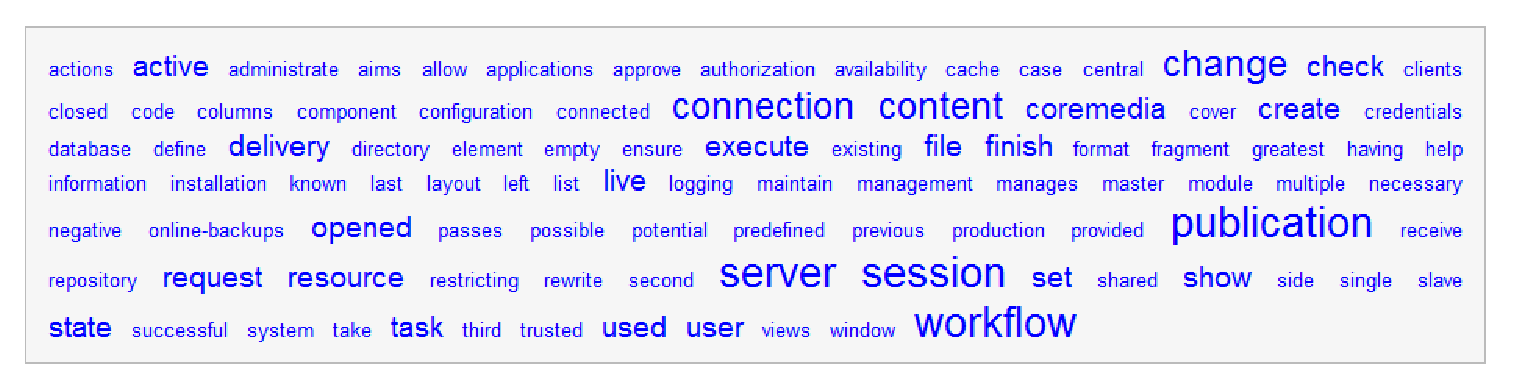
\includegraphics[width=\ScaleIfNeeded]{img/tagcloud} 
 % or [scale=0.5]
	\caption{Tag Cloud}
	\label{fig:tagcloud}
\end{figure}

\section{1}
\label{sec:semannot:1}
Related work 
SenseBot Search Results Summarizer is a plugin for Mozilla Firefox browser that generates a tag cloud of the main concepts returned as search results from Google.

LinkSensor
SenseBotSummarizer
All three are based on SenseBot - a semantic search engine.
Made available from Semantic Firefox Extensions \footnote{\url{http://www.semanticengines.com/plugins.htm}}

\chapter{Implementation}
\label{sec:implementation}

This chapter describes the implementation part of the thesis work. After presenting in Chapter~\ref{sec:lsa} the theoretical basis behind \gls{LSA}, and in Chapter~\ref{chapter:cluster_labeling} cluster labeling, theoretical application and specific implementation decisions are discussed here. All software tools and libraries which were used are pointed out, and code snipplets are given. Then in Chapter~\ref{chapter:evaluation}, test results are shown, and evaluation of the implementation is made. \\

\section{Clustering, labeling}
For the ontology development, we used Protege Ontology Editor 4.1~\footnote{\url{http://protege.stanford.edu/}, accessed December, 2010} from Stanfornd University. The ontology is a light-weight domain-specific ontology developed in OWL for CoreMedia \gls{CMS} domain. \\

\section{Tag Cloud implementation}
\label{sec:implementation:tag_cloud}
The implemented open source library used for tag cloud generation is called Opencloud\footnote{\url{http://opencloud.mcavallo.org/}, accessed December, 2010}, and is provided by Marco Cavallo.\\

Tag clouds can be generated automatically by using the most frequent words, by removing stop words, etc. preprosessing. They can also be custom made, by using important concepts retrieved after \gls{IR} task has been performed - e.g. on search results, on main concepts as in our case, based on concepts retrieved using \gls{LSA}. \\

\section{Tools used}
\label{sec:implementation:tools_used}
Airhead Research\footnote{\url{http://code.google.com/p/airhead-research/}} project was used as a semantic spaces Package which provides a java-based implementation of \gls{LSA}.\\

Apache Lucene\footnote{\url{http://lucene.apache.org/java/3_0_2/}, accessed December, 2010} was used as an indexing and search library.

\section{Advantages and drawbacks}
\label{sec:lsa:adv_disadv}

why am i using lsa instead of lda for example?\\

\begin{enumerate}
\item PLSA - characteristics, advantages, disadvantages
\item LDA - characteristics, advantages, disadvantages
\end{enumerate}


\chapter{Evaluation}
\label{chapter:evaluation}

Evaluation in \gls{IR} is based on measures. As this work implements techniques for information retrieval, several wide-spread measures are described next, used commonly in \gls{IR} systems to evaluate performance. Then, the implemented tests are presented, and finally are discussed the obtained test results. \\


\section{Measures for evaluation}
If an evaluation of \gls{IR} systems is performed, one needs in the simplest case:
\begin{itemize}
\item a document collection, 
\item a test suite of information needs, or a set of queries,
\item a set of relevance judgments to define for each query-document pair weather the document is relevant or not relevant for the query posed.
\end{itemize} 

Relevance is assessed relative to an information need, not a query. A document is considered relevant if it addresses the users' information need, not only if it contains all the words given in the query~(Manning et al.~\cite{Mann08}). When short queries (composed of one word for example) are posted, it is difficult to define the information need of users. But nevertheless, the user has one, and the retrieved search results are evaluated based on his or her information need. \\

The two most frequent and basic measures for evaluation of \gls{IR} systems are \textit{precision} and \textit{recall}. For the simple case of a system which returns a result set of document to a query, they are defined:  \\

\subsubsection{Precision}
\subsubsection{Recall}


\subsection{Evaluation of LSA}
Presision: \\
Recall: \\

\subsection{Evaluation of algorithms for cluster labeling}
User evaluation of cluster labeling algorithm \\
? F-measure:\\

\section{Experimental evaluation}
Example for presentation and evaluation of results, IR system:~\cite{SpamFilteringLSI2008} \\
\begin{itemize}
\item Data set
\item Experimental setup
\item Analysis of data matrices
\item True/false positive rates
\item Feature reduction
\end{itemize}

\section{LSA implementation}
\label{sec:implementation:lsa_impl}
\gls{LSA} was applied to a collection of 11818 words in 4000 documents, all of which describe CoreMedia \gls{CMS} 5.2. The algorithm took 63552 ms for preprocessing and indexing of the whole document collection. \\

For the implementation of LSA this work uses the open LSA library which is part of Semantic Spaces Project\cite{S-Space}. It is developed at the Natural Language Processing Group at the University of California at Berkley (UCLA)\footnote{\url{http://code.google.com/p/airhead-research/}, accessed December, 2010}.\\

The real difficulty of LSA is to find out how many dimensions to remove - the problem of dimensionality.\\

TODO:test if inluding only terms that occur in more than one document improved \gls{LSA} performance with respect to generating precise tag clouds.\\

\subsubsection{Data set}
It is a challenge by itself to come up with a sensible evaluation set for an IR implementation. ... Define here precision, recall, measures , how to measure LSA performance with  diff. k, clusters, cluster labelling. \\

The document collection consists of guides and manuals about CoreMedia \gls{CMS} 5.2.\\

This work has been carried out using documents from the domain of CoreMedia \gls{CMS} 5.2 as an evaluation set, developed at CoreMedia AG, Hamburg. \\


\subsubsection{Data preprocessing}
Stop words and punctuation are removed. The data model used in DocMachine stores the documents as XML files, and CoreMedia \gls{CMS} Unified API\footnote{\url{https://documentation.coremedia.com/servlet/content/241548?language=en&version=5.2&book=coremedia:///cap/content/241548}} is used to strip the markup, in order to access the plain text~(listing~\ref{strip_markup}). \\

\section{Cluster labeling}

The experiments in this study conducted several objective measures to validate the performance of the described algorithm \gls{WCC}. \\

Evaluating the quality of cluster labeling is a non-trivial task and the most suitable evaluation is judged by user's experiences. \\

The algorithm was implemented in Java on a a 64-bit Windows 7 Ultimate workstation with an Intel Core 2 Duo P8600 @ 2,40 GHz using 4.00 GB RAM. \\

\subsubsection{Document set}
In order to test a cluster labeling algorithm, we need a test data set containing predefined categories. \gls{WCC} is tested using the evaluation data set with three predefined categories selected from the whole collection used for evaluation of \gls{LSA} implementation. \\
 
\begin{table}[]
\centering
\begin{tabular}{l l  c}
\hline
\multicolumn{3}{c}{Document set overview}\\
\hline
Category Id & Category & Document \# \\
\hline
1 & session, connection & 5 \\
2 & server & 5 \\
3 & publication, workflow & 5 \\
\hline
\end{tabular}
\caption[Document set overview]{Overview of the constructed document set}
\end{table}

The document set used for evaluation consists of 3 categories, and 15 documents - each category has 5 documents, and the documents have different length. Table~\ref{eval:data_set} gives an overview of the constructed data sets. The document preprocessing involves parsing and stop word removal according to standard stop word lists. \\


\textbf{Data preprocessing} \\
The evaluation document set needs to be preprocessed before it can be used in the experiments. Analogous to the preprocessing used for the whole data set, punctuation and stop-words were removed. Terms in texts were not stemmed, as they are used as cluster labels, and stemming the terms would lead to worse user experience. \\

% TODO: correct text wrapping - fix column width for document text
%\begin{landscape}
\begin{table} [!ht]
\centering
\begin{tabular} { c c p{10cm} }
\hline
Doc. Id & Cat. Id & Document \\
\hline
1 & 1 & The session that is created while the connection is opened is also known as the connection session. \\
2 & 1 & The sessions of the connected clients will be closed and no more content changes are possible. \\
3 & 1 & The previous code fragment shows how a second session is created from an existing connection. \\
4 & 1 & Multiple sessions show their greatest potential in trusted applications which receive help in restricting user views while maintaining a shared cache.  \\
5 & 1 & Having opened connection, all actions are executed on behalf of the single user whose credentials where provided when logging in. \\
\hline
6 & 2 & The state of the Master Live Server must be younger than the state of the Slave Live Server.  \\
7 & 2 & The rewrite module checks the availability of the requested file and, in the negative case, passes the request on to the Active Delivery Server. \\
8 & 2 & The directory layout of the Active Delivery Server has changed as well as the format of the configuration file. \\
9 & 2 & The CoreMedia Content Server is a central component that manages the content repository and the user authorization. \\
10 & 2 & The CoreMedia Content Management Server is the production system used to create and administrate content. \\
\hline
11 & 3 & If the database does not allow to take online-backups ensure that all publications are finished and that the last publication was successful. \\
12 & 3 & The third task in the workflow aims to check if the change set is empty. Then, no publication is necessary and the workflow can be finished.  \\
13 & 3 & This element is used to define which information should be shown in the columns of the workflow list at the left side of the workflow window. \\
14 & 3 & Publication will be executed when finishing the task after all resources in the change set have been approved. \\
15 & 3 & The CoreMedia Workflow installation comes with four predefined workflows which cover the publication of resources. \\
\hline
\end{tabular}
\caption[Document collection used for WCC testing]{Document collection used for WCC testing}
\label{eval:data_set}
\end{table}


\subsection{Cluster labeling evaluation}

To evaluate the quality of WCC, Popescul and Ungar�s method, and the standard
keyword extraction algorithm RSP, we downloaded 150 documents from the digital library Citeseer, each of which containing author-defined keywords.

To evaluate the WCC algorithm, we prepared a document set with author-defined keywords. The evaluation idea is to cluster the documents, label the resulting clustering, compute f1-f4, and measure to which extent the identified topic labels appear in the keyword list of at least one document of the associated cluster. To measure the extent, standard precision and recall values can be chosen. Note, however, that the precision value is more important in our scenario since usually only a few words (about one to five) are presented to a user. \\

The clustering was done on the results from queries used for evaluation of \gls{LSA} (??).  \\
The clustering was done on the prepared data set~\ref{eval:data_set}, used for evaluation of the \gls{IR} methods implemented in this work. \\

Figure 3.15 shows precision and recall curves for \gls{WCC} depending on the number of extracted words per label. The values are averaged over 10 retries of the experiment, each time redrawing a new set of documents. The precision curve shows that one to five cluster labels can be identified at very high precision rates. (??check with my results?) \\


\section{LSA evaluation from IR book}
� The computational cost of the SVD is significant. This has been the biggest obstacle to the widespread adoption to LSI. One approach to this obstacle is to build the LSI representation on a
randomly sampled subset of the documents in the collection, following which the remaining documents are �folded in� as detailed with Equation (18.21). \\
� As we reduce k, recall tends to increase, as expected. \\
� Most surprisingly, a value of k in the low hundreds can actually increase
precision on some query benchmarks. This appears to suggest that for a
suitable value of k, LSI addresses some of the challenges of synonymy. \\
� LSIworks best in applicationswhere there is little overlap between queries
and documents. \\
The experiments also documented some modes where LSI failed to match
the effectiveness of more traditional indexes and score computations. Most
notably (and perhaps obviously), LSI shares two basic drawbacks of vector
space retrieval: there is no good way of expressing negations (find documents
that contain german but not shepherd), and noway of enforcing Boolean
conditions. \\
LSI can be viewed as soft clustering by interpreting SOFT CLUSTERING each dimension of the
reduced space as a cluster and the value that a document has on that dimension
as its fractional membership in that cluster. \\


\chapter{Conclusion and outlook}
\label{sec:conclusion}

Search applications process huge amounts of information. Presenting this information to the users is an important part of these applications, and can improve their usability. We applied clustering as a method to organize search results into browsable groups of documents. In order to present these prepared groups of documents to the end users, informative and summarizing cluster labels are needed. Therefore, we evaluated the implementation of \gls{WCC} cluster labeling method, and outlined a proposal for its improvement. \\

With respect to the problem of how to present many search results to users, we implemented a tag cloud, which summarizes the main concepts in search results, thus acting as a visualization mean. 


\section{Future Work}
The goals set for this project and given in section~\ref{sec:goal_scope} were reached. The project can still be developed further. Below, we outline our proposals for future work. \\

\subsection{Implementation}

! Implement the prototype as a part of DocMachine\footnote{\url{https://documentation.coremedia.com/}} - the online documentation system at CoreMedia AG, Hamburg.

\subsubsection{LSA}
One of the major drawbacks in implementing \gls{LSA} is that computing \gls{SVD} for large matrices when applied to large document sets is computationally expensive. It has been stated that it is possible to compute \gls{SVD} in an incremental manner, and with reduced resources via neural-network like approach~\cite{brand06}. However, currently there is no Java-based implementation of this algorithm. As this project is developed using Java, it remains as future work to implement the fast incremental \gls{SVD} computation, proposed by Brand~\cite{brand06} in Java, in order to use it in this work. \\

\subsubsection{Cluster labeling}
Other clustering methods can be investigated, such as \gls{STC}, which preserves the word order in documents, by presenting them in the form of a tree. Cluster labeling using \gls{STC} involves also using phrases as candidate labels, instead of separate terms, which improves usability, as compared 
to the investigates \gls{WCC} algorithm. \\

\subsubsection{Cluster labeling using external knowledge}
Due to time constraints, it remains for future work to evaluate and present experimental results on running \gls{WCC} algorithm for cluster labeling with external knowledge from an ontology. \\

\subsection{Testing}
A larger set of document can be used for evaluation and testing of our implementation. In this work we carried out tests on a document set consisting only of 15 documents in 3 categories. Research has shown, however, that \gls{LSA} perform better when applied to document collections above 3000 documents, each of which larger than $\approx 60$ words, testing our implementation on a larger document collection remains as future work. \\


% prints the list of acronyms
% call: latex thesis, makeglossaries thesis, latex thesis
\printglossaries


\begin{appendix}
\chapter{Ontology}
\label{appendix:onto}

\begin{figure}[H]
%  \resizebox{\textwidth}{!}{\rotatebox{90}{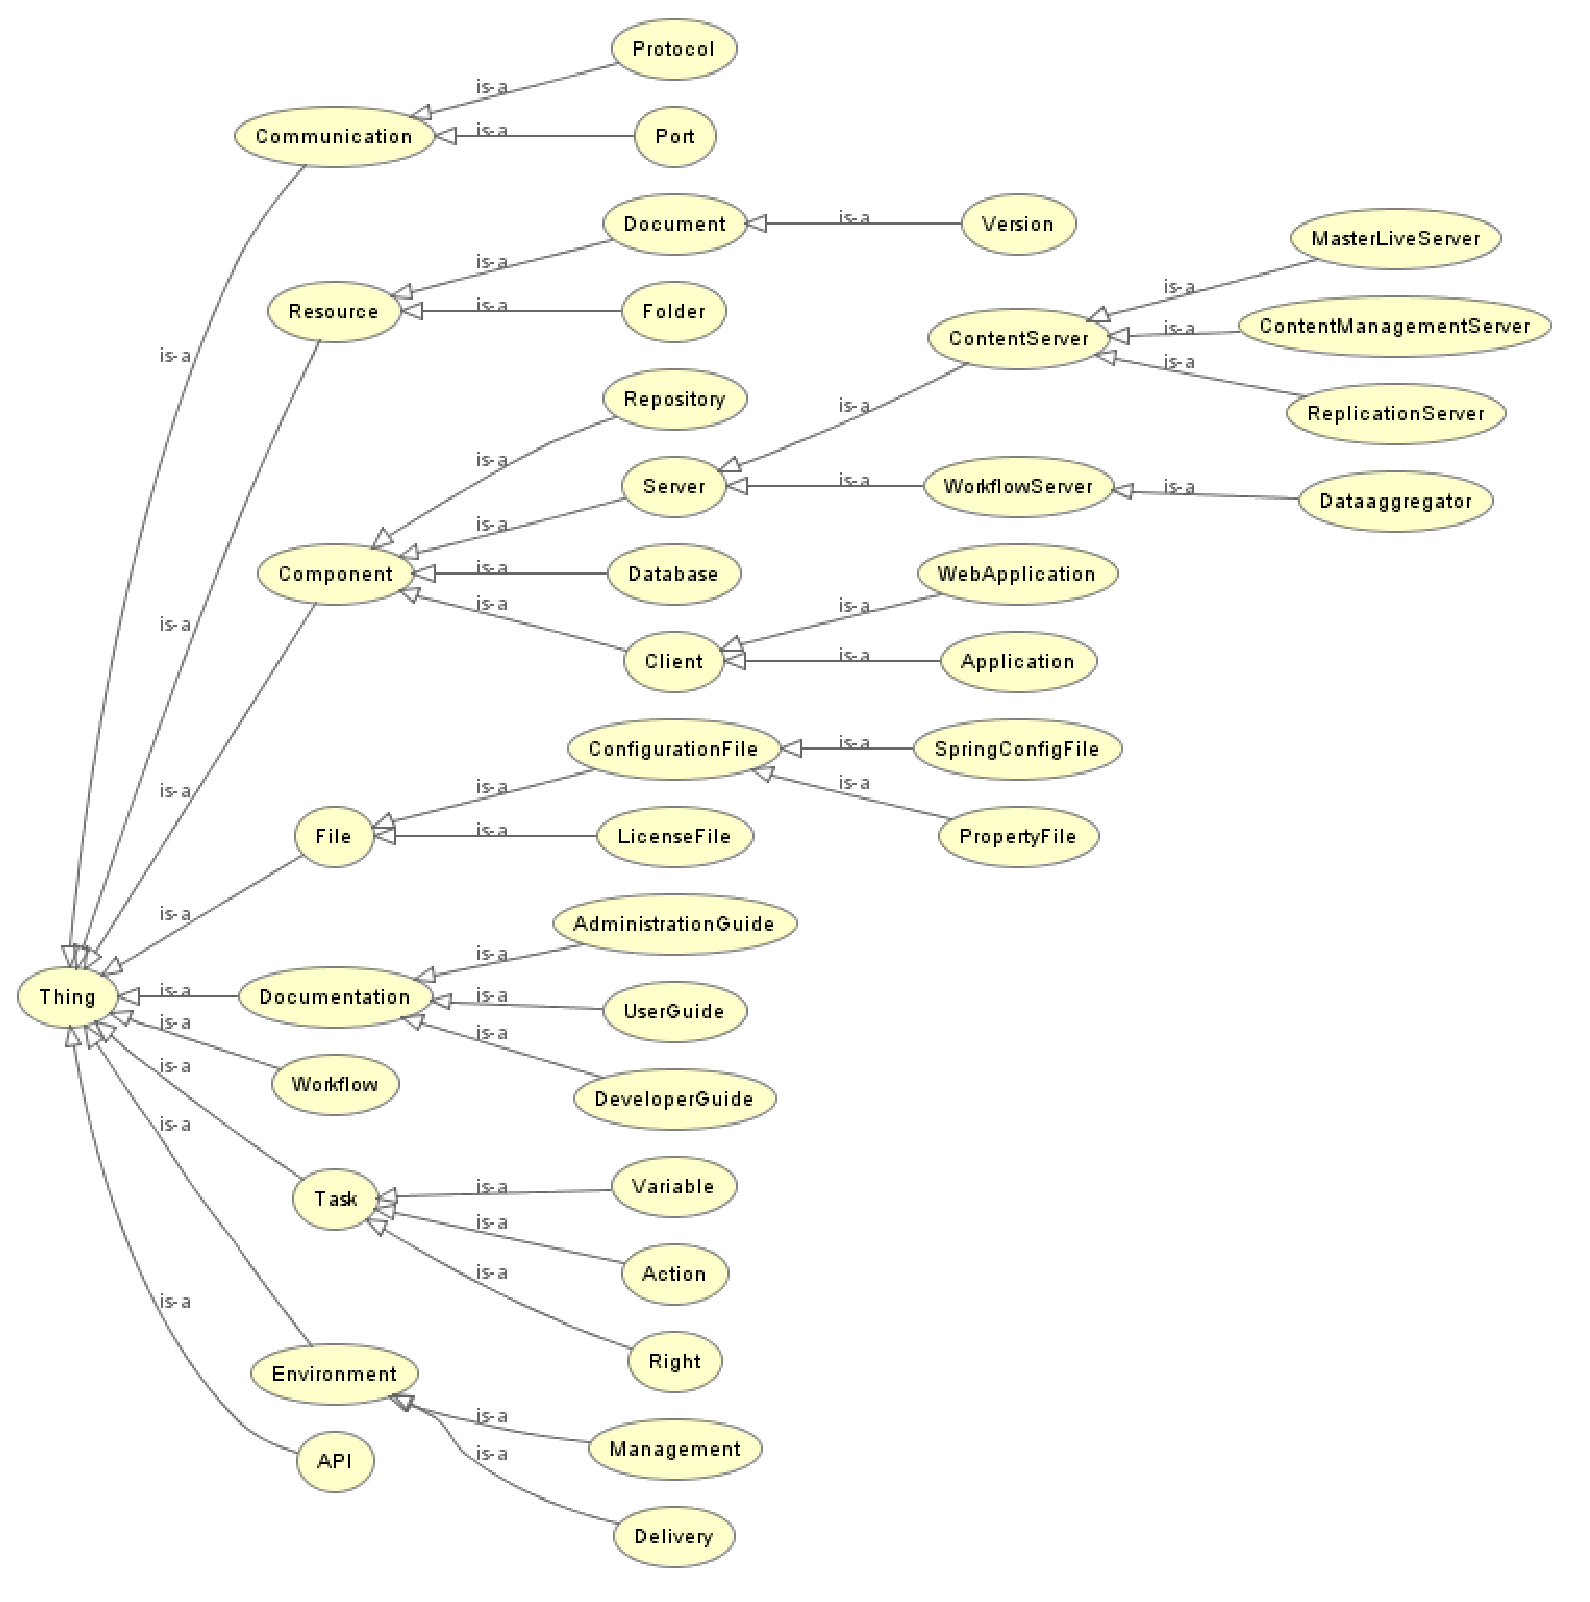
\includegraphics{img/CoreMediaOntology}}}
  \resizebox{\textwidth}{!}{{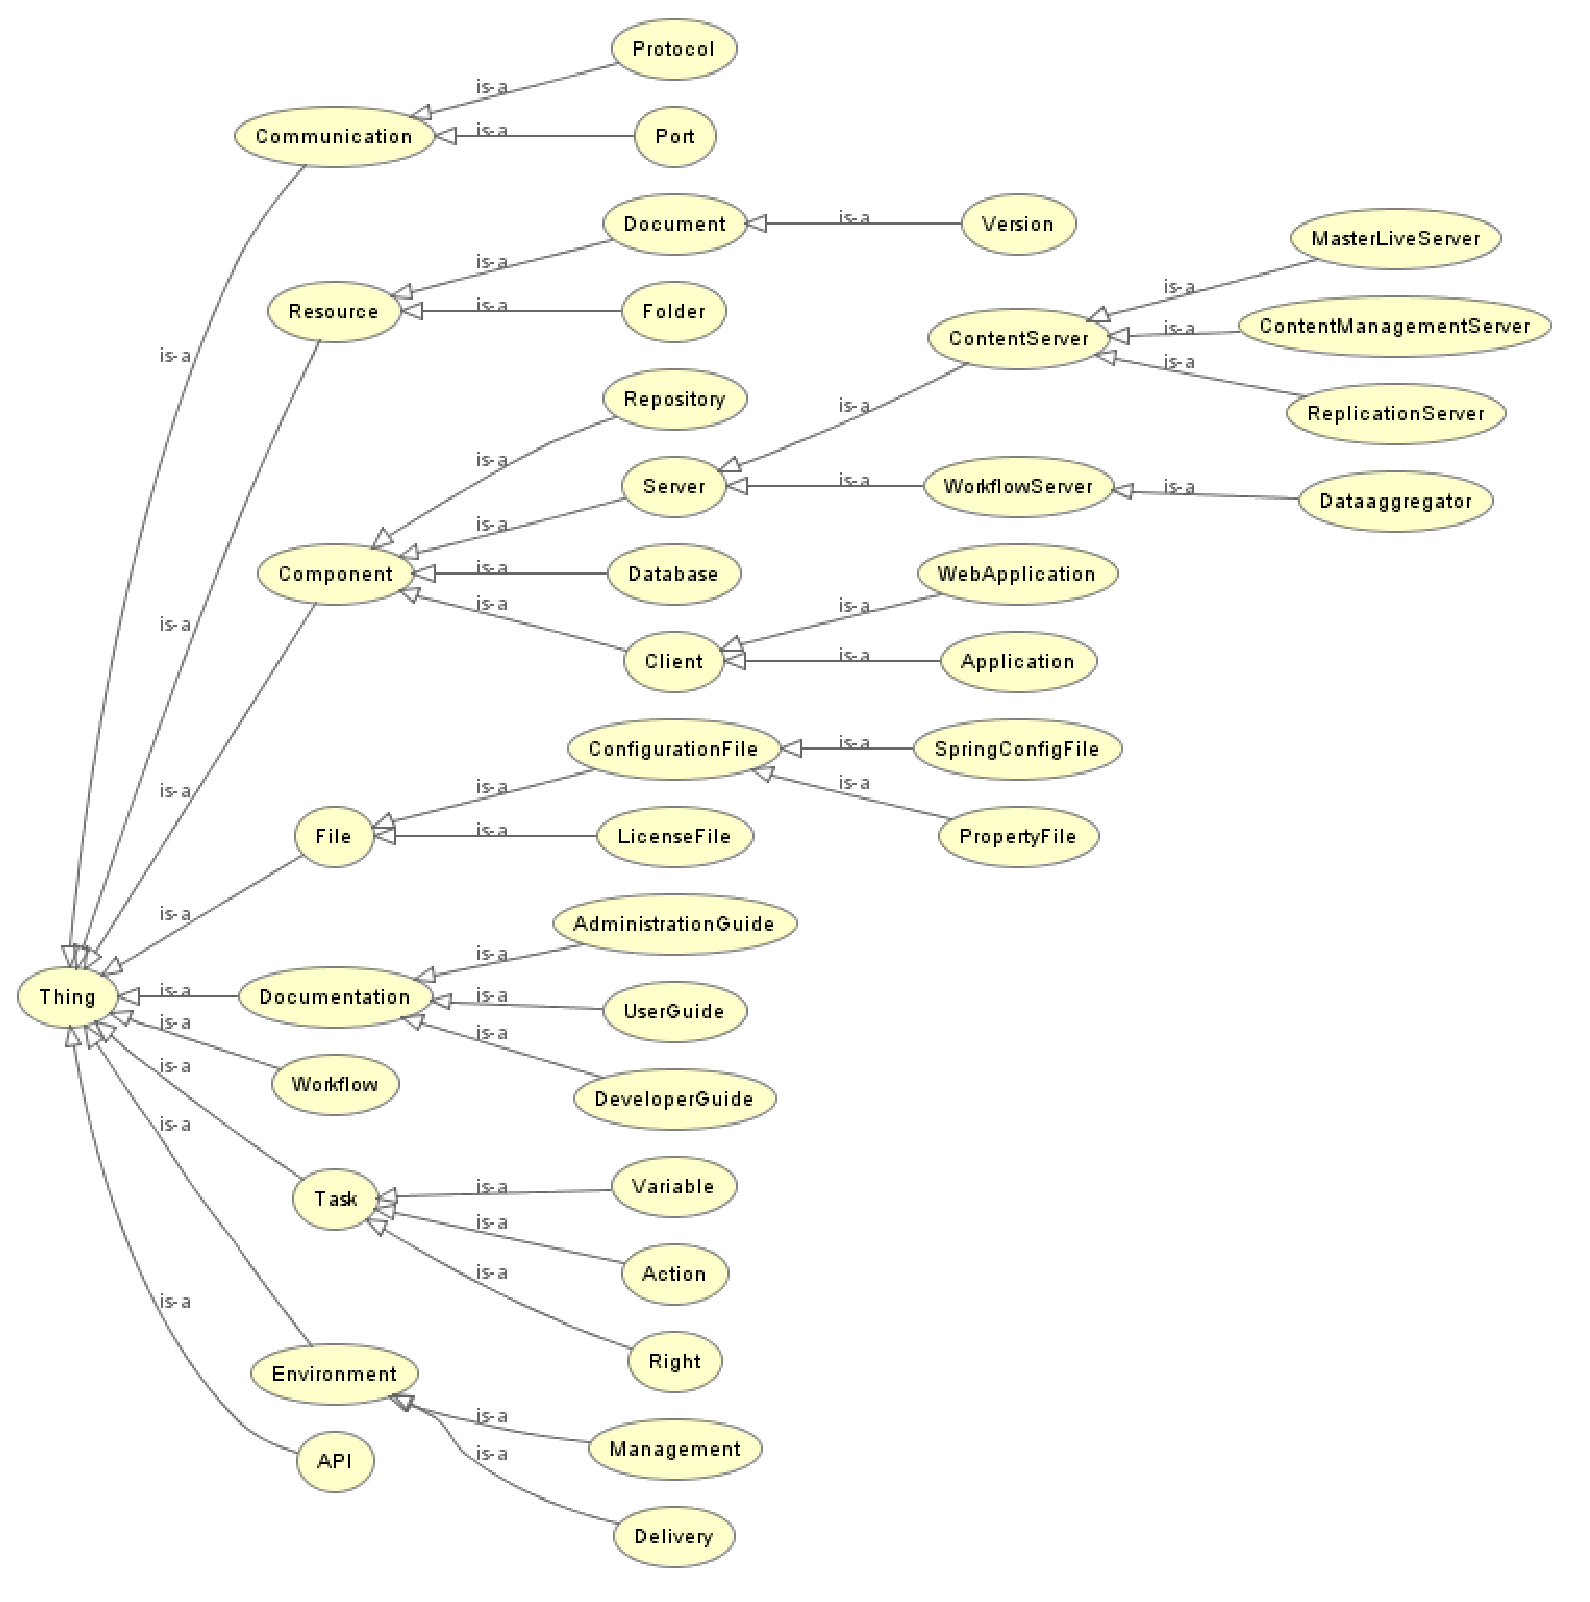
\includegraphics{img/CoreMediaOntology}}}
  \caption[Upper level domain specific ontology]%
          {Upper level ontology for CoreMedia \gls{CMS} domain}
  \label{appendix:ontology}
\end{figure}

\chapter{Source code}

\lstinputlisting[label=doc_preprocessing,caption=Preprocessing of the document collection - markup is stripped from plain text]{code/ProcessDocuments.java}

\pagebreak

\lstinputlisting[label=code_lat_analysis,caption=Latent Semantic Analysis]{code/LSA.java}

\pagebreak

\lstinputlisting[label=querying,caption=Querying the semantic space\, constructed by LSA]{code/Query.java}

\pagebreak

\lstinputlisting[label=tag_cloud,caption=Tag cloud generation]{code/TagCloud.java}

\pagebreak

\lstinputlisting[label=topic_identification,caption=WCC cluster labeling algorithm]{code/TopicIdentification.java}

\pagebreak

\lstinputlisting[label=cm_ontology,caption=Lightweight domain ontology for CoreMedia CMS domain]{code/CoreMediaCMS.owl}

\end{appendix}

% number the bibliography instead of alpha-numerical abbrev.
%\bibliographystyle{alpha} 
\pdfbookmark[0]{Bibliography}{references}
\bibliographystyle{ieeetr}
\bibliography{references}

\end{document}
